% APCCM2017_Stanger.tex
% Author: Nigel Stanger
%
% Built using Tex Live 2016 distribution.
% All packages except perhaps PGF should be in the standard TeX Live packages.
% REQUIRES PGF v3.0 or later for diagrams (custom arrow tips).
% REQUIRES TeX Gyre fonts (newtxmath package).
% NOTE: the last two figures use a small amount of colour.
%
% Revisions: 22 Aug 2016 Initial submission.
%            07 Nov 2016 Camera-ready version.

%%
%% MAX 10 PAGES (all material)
%%

\documentclass{sig-alternate-05-2015}

\usepackage{balance}
\usepackage{newtxtext}
\usepackage{newtxmath}
\usepackage{bm}
\usepackage{subfig}
\usepackage{booktabs}

\usepackage{tikz}
\usetikzlibrary{positioning}
\usetikzlibrary{graphs}
\usetikzlibrary{decorations.pathreplacing}
\usetikzlibrary{calc}
\usetikzlibrary{arrows}


% Relational algebra operators
\newcommand{\RelRestrict}{\ensuremath{\sigma}}
\newcommand{\RelProject}{\ensuremath{\pi}}
\newcommand{\RelUnion}{\ensuremath{\cup}}
\newcommand{\RelIntersect}{\ensuremath{\cap}}


% "empty" arrow tip
\pgfarrowsdeclare{:}{:}{}{}
% custom bar arrow tip, offset from end of line (use "empty" tip at line ends if no >)
\tikzset{crossbar/.tip={|[scale width=1.75,sep=0.25em]}}
% various edge styles for SIG diagrams in TikZ
\tikzset{
    function/.style={arrows={->}},
    injection/.style={arrows={<-}},
    total/.style={arrows={:{crossbar}-}},
    surjection/.style={arrows={-{crossbar}:}},
    bijection/.style={arrows={<{crossbar}-{crossbar}>}},
    projection/.style={arrows={:{crossbar}-{crossbar}>}},
    projection left/.style={arrows={:{crossbar}-{crossbar}>},edge label={\scriptsize\(\RelProject\)}},
    projection right/.style={arrows={:{crossbar}-{crossbar}>},edge label'={\scriptsize\(\RelProject\)}},
    selection left/.style={arrows={<-{crossbar}>},edge label={\scriptsize\(\RelRestrict\)}},
    selection right/.style={arrows={<-{crossbar}>},edge label'={\scriptsize\(\RelRestrict\)}},
    funcdep left/.style={arrows={:{crossbar}-{crossbar}>},edge node={node[sloped,midway,above] {\scriptsize\emph{key}}}},
    funcdep right/.style={arrows={:{crossbar}-{crossbar}>},edge node={node[sloped,midway,below] {\scriptsize\emph{key}}}},
    surtotal/.style={arrows={:{crossbar}-{crossbar}:}},
    input keep/.style={blue,thick},
    input delete/.style={blue!40,thick,dashed},
    output/.style={red,thick},
    output temp/.style={red,thick,dashed},
    path 1/.style={green!60!black,thick},
    path 2/.style={orange,thick},
}
        
% projection and selection edge annotations for TikZ
\newcommand{\ProjectionAnnotation}[3][]{%
    \path (#2) to node[above,#1] {\scriptsize\(\RelProject\)} (#3);%
}
\newcommand{\SelectionAnnotation}[3][]{%
    \path (#2) to node[above,#1] {\scriptsize\(\RelRestrict\)} (#3);%
}


\newcounter{constraint}

% misc
% \newcommand{\todo}[1]{\textbf{!!TODO!!} {[#1]}}

% commonly used elements
\newcommand{\LS}{\ensuremath{\mathit{LS}}}
\newcommand{\NLS}{\ensuremath{\mathit{NLS}}}
\newcommand{\LSsub}{\ensuremath{\mathit{L}}}
\newcommand{\NLSsub}{\ensuremath{\mathit{N}}}
\newcommand{\Sno}{\ensuremath{\mathit{Sno}}}
\newcommand{\Sname}{\ensuremath{\mathit{Sname}}}
\newcommand{\Status}{\ensuremath{\mathit{Status}}}
\newcommand{\City}{\ensuremath{\mathit{City}}}

\newcommand{\Type}[1]{\ensuremath{T_{#1}}}
\newcommand{\TT}[1]{\ensuremath{T_{\{#1\}}}}

\newcommand{\CityLondon}{\ensuremath{\{\City\colon\allowbreak\text{`\emph{London}'}\}}}
\newcommand{\TCityMinusLondon}{\ensuremath{\Type{\City} \setminus \CityLondon}}
\newcommand{\TSSC}{\ensuremath{\Type{\Sname} \times \Type{\Status} \times \Type{\City}}}
\newcommand{\TSSL}{\ensuremath{\Type{\Sname} \times \Type{\Status} \times \CityLondon}}
\newcommand{\TSSNL}{\ensuremath{\Type{\Sname} \times \Type{\Status} \times (\TCityMinusLondon)}}

\newcommand{\TLSPlusNLS}{\ensuremath{\Type{\LS} + \Type{\NLS}}}
\newcommand{\TTLSPlusNLS}{\ensuremath{\TT{\LS} + \TT{\NLS}}}
\newcommand{\TLSPlusNLSsub}{\ensuremath{\Type{\LSsub} + \Type{\NLSsub}}}
\newcommand{\TTLSPlusNLSsub}{\ensuremath{\TT{\LSsub} + \TT{\NLSsub}}}

\newcommand{\StackTLSPlusNLS}{\ensuremath{\begin{array}{c}\Type{\LS}\,+ \\ \Type{\NLS}\end{array}}}
\newcommand{\StackTTLSPlusNLS}{\ensuremath{\begin{array}{c}\TT{\LS}\,+ \\ \TT{\NLS}\end{array}}}
\newcommand{\StackTLSPlusNLSsub}{\ensuremath{\begin{array}{c}\Type{\LSsub}\,+ \\ \Type{\NLSsub}\end{array}}}
\newcommand{\StackTTLSPlusNLSsub}{\ensuremath{\begin{array}{c}\TT{\LSsub}\,+ \\ \TT{\NLSsub}\end{array}}}
\newcommand{\StackTSSC}{\ensuremath{\begin{array}{c}\Type{\Sname}\,\times \\ \Type{\Status} \times \Type{\City}\end{array}}}
\newcommand{\StackTSSL}{\ensuremath{\begin{array}{c}\Type{\Sname} \times \Type{\Status}\,\times \\ \CityLondon\end{array}}}
\newcommand{\StackTSSNL}{\ensuremath{\begin{array}{c}\Type{\Sname} \times \Type{\Status}\,\times \\ (\TCityMinusLondon)\end{array}}}
\newcommand{\StackTCityMinusLondon}{\ensuremath{\begin{array}{c}\Type{\City}\,\setminus \\ \CityLondon\end{array}}}

\newcommand{\SC}[1]{\ensuremath{\mathcal{S}_{#1}}}

% dominates
\newcommand{\Dominates}[2]{\ensuremath{#2 \preceq #1}}
\newcommand{\Equivalent}[2]{\ensuremath{#1 \equiv #2}}

% SIG notation (in text)
\newcommand{\Sedge}[1]{\ensuremath{\sigma_{\textrm{#1}}}}
\newcommand{\SedgeP}[1]{\ensuremath{\sigma_{\textrm{#1}}^{'}}}

\newcommand{\medmid}{\raise.125ex\hbox{\scalebox{1}[0.75]{$\mid$}}}

% General SIG edges for use in formulas.
% Adapted from: http://tex.stackexchange.com/questions/96330/adding-symbols-at-the-ends-of-a-horizontal-line
\makeatletter
\newlength{\@annotskipleft}
\newlength{\@annotskipright}
% #1 = left edge component
% #2 = right edge component
% #3 = left bar annotation
% #4 = right bar annotation
\newcommand\@sig@edge[4]{%
    \let\@middle\joinrel%
    \ifx#1\relbar%
        \@annotskipleft=.3em%
        % scrunch up the bare line so it's similar length to \long...arrow
        \ifx#2\relbar\def\@middle{\joinrel\joinrel\relbar\joinrel\joinrel}\fi%
    \else% 
        % arrows need a little more clearance
        \@annotskipleft=.4em%
    \fi%
    \ifx#2\relbar\@annotskipright=.3em\else\@annotskipright=.4em\fi%
    \mathrel{\ooalign{$#1\@middle#2$\cr\hskip\@annotskipleft$#3$\hfil$#4$\hskip\@annotskipright\cr}}%
}

% 0 = nothing
% 1 = bar
% 2 = arrowhead
% 3 = both
\def\@sigedge#1#2{%
    \ifcase\numexpr#1*4+#2\relax%
        \@sig@edge{\relbar}{\relbar}{}{}\or                     % 00 = -----
        \@sig@edge{\relbar}{\relbar}{}{\medmid}\or              % 01 = ---+-
        \@sig@edge{\relbar}{\rightarrow}{}{}\or                 % 02 = ---->
        \@sig@edge{\relbar}{\rightarrow}{}{\medmid}\or          % 03 = ---+>
        \@sig@edge{\relbar}{\relbar}{\medmid}{}\or              % 10 = -+---
        \@sig@edge{\relbar}{\relbar}{\medmid}{\medmid}\or       % 11 = -+-+-
        \@sig@edge{\relbar}{\rightarrow}{\medmid}{}\or          % 12 = -+-->
        \@sig@edge{\relbar}{\rightarrow}{\medmid}{\medmid}\or   % 13 = -+-+>
        \@sig@edge{\leftarrow}{\relbar}{}{}\or                  % 20 = <----
        \@sig@edge{\leftarrow}{\relbar}{}{\medmid}\or           % 21 = <--+-
        \@sig@edge{\leftarrow}{\rightarrow}{}{}\or              % 22 = <--->
        \@sig@edge{\leftarrow}{\rightarrow}{}{\medmid}\or       % 23 = <--+>
        \@sig@edge{\leftarrow}{\relbar}{\medmid}{}\or           % 30 = <+---
        \@sig@edge{\leftarrow}{\relbar}{\medmid}{\medmid}\or    % 31 = <+-+-
        \@sig@edge{\leftarrow}{\rightarrow}{\medmid}{}\or       % 32 = <+-->
        \@sig@edge{\leftarrow}{\rightarrow}{\medmid}{\medmid}   % 33 = <+-+>
    \fi%
}

\newcommand{\sigedge}[1]{\ensuremath{\@sigedge#1}}
\makeatother

\newcommand{\Edge}{\sigedge{00}}
\newcommand{\Total}{\sigedge{10}}
\newcommand{\Surjective}{\sigedge{01}}
\newcommand{\SurTotal}{\sigedge{11}}
\newcommand{\Functional}{\sigedge{02}}
\newcommand{\Injective}{\sigedge{20}}
\newcommand{\Bijective}{\sigedge{33}}

% Hack to get the overset symbols to appear at the right height.
% \smash removes the spacing around the operator, hence \mathop.
\newcommand{\LabelledEdge}[2]{\mathop{\overset{\raisebox{0.3em}{\scriptsize\ensuremath{#2}}}{\smash[t]{#1}}}}
\newcommand{\ProjectionEdge}{\LabelledEdge{\sigedge{13}}{\RelProject}}
\newcommand{\SelectionEdge}{\LabelledEdge{\sigedge{23}}{\RelRestrict}}
\newcommand{\TrivialProjection}{\ensuremath{\LabelledEdge{\Bijective}{\RelProject}}}
\newcommand{\TrivialSelection}{\ensuremath{\LabelledEdge{\Bijective}{\RelRestrict}}}
\newcommand{\KeyEdge}{\ensuremath{\LabelledEdge{\sigedge{13}}{\mathit{key}}}}

% Constraints.
\newcommand{\Constraint}[2][]{C\ensuremath{_{#2}\ifx&#1&\else^{#1}\fi}}
\newenvironment{ConstraintList}[1][]{%
    \begin{list}{%
        \bfseries%
        \ifx&#1&%
            \Constraint{\ensuremath{\bm{\arabic{constraint}}}}%
        \else%
            \Constraint[\ensuremath{\bm{#1}}]{\ensuremath{\bm{\arabic{constraint}}}}%
        \fi%
    }%
    {\usecounter{constraint}}%
}{\end{list}}


\hyphenation{co-pied sche-ma}

\pagestyle{empty}


%%%%%%%%%%%%%%%%%%%%%%%%%%%%%%%%%%%%%%%%%%%%%%%%%%%%%%%%%%%%%%%%%%%%%%%%%%%%%%%%%


\begin{document}

\CopyrightYear{2017} 
\setcopyright{acmlicensed}
\conferenceinfo{ACSW '17,}{January 31-February 03, 2017, Geelong, Australia}
\isbn{978-1-4503-4768-6/17/01}\acmPrice{\$15.00}
\doi{http://dx.doi.org/10.1145/3014812.3014847}

\title{Characterising relational view updates \\ using relative information capacity}

\numberofauthors{1}
\author{
\alignauthor Nigel Stanger \\
    \affaddr{Department of Information Science, University of Otago}\\
    \affaddr{Dunedin, New Zealand}\\
    \email{nigel.stanger@otago.ac.nz}
}

\begin{CCSXML}
<ccs2012>
<concept>
<concept_id>10002951.10002952.10002953.10002955</concept_id>
<concept_desc>Information systems~Relational database model</concept_desc>
<concept_significance>500</concept_significance>
</concept>
<concept>
<concept_id>10002951.10002952.10003190.10003205</concept_id>
<concept_desc>Information systems~Database views</concept_desc>
<concept_significance>500</concept_significance>
</concept>
<concept>
<concept_id>10003752.10010070.10010111.10010112</concept_id>
<concept_desc>Theory of computation~Data modeling</concept_desc>
<concept_significance>300</concept_significance>
</concept>
<concept>
<concept_id>10003752.10010070.10010111.10011733</concept_id>
<concept_desc>Theory of computation~Data integration</concept_desc>
<concept_significance>300</concept_significance>
</concept>
</ccs2012>
\end{CCSXML}

\ccsdesc[500]{Information systems~Relational database model}
\ccsdesc[500]{Information systems~Database views}
\ccsdesc[300]{Theory of computation~Data modeling}
\ccsdesc[300]{Theory of computation~Data integration}

\maketitle


%%%%%%%%%%%%%%%%%%%%%%%%%%%%%%%%%%%%%%%%%%%%%%%%%%%%%%%%%%%%%%%%%%%%%%%%%%%%%%%%%


\begin{abstract}
In 2013, Chris Date published a book about the view update problem in the context of the Relational Model. He presented several detailed examples of different varieties of view updates and characterised their behaviour, in the process deriving a set of principles for updating views based on the notion of \emph{information equivalence} of view schemas. In this paper we discuss work in progress that examines how Date's operational definition of information equivalence can be formally characterised using Hull's concept of \emph{relative information capacity}. As a proof of concept, we use an extension of Miller's \emph{schema intension graph} formalism to model the information equivalence of Date's restriction view example.
\end{abstract}


%%%%%%%%%%%%%%%%%%%%%%%%%%%%%%%%%%%%%%%%%%%%%%%%%%%%%%%%%%%%%%%%%%%%%%%%%%%%%%%%%


\keywords{view update problem, information equivalence, relative information capacity, schema intension graph, schema transformation}


%%%%%%%%%%%%%%%%%%%%%%%%%%%%%%%%%%%%%%%%%%%%%%%%%%%%%%%%%%%%%%%%%%%%%%%%%%%%%%%%%


\section{Introduction}

\noindent The view update problem is a long-standing problem of great practical significance in the database field. Date \cite{Date.C-2013a-View} likens it to significant unsolved problems in other fields such as the Riemann Hypothesis in mathematics or ``\(P = \mathit{NP}\)?'' in computational complexity theory. In his 2013 book \cite{Date.C-2013a-View} Date developed a set of principles for updating relational views, based on the notion of \emph{information equivalence}. However, that notion was defined more operationally than formally.

View updating is a special case of schema translation: we have one schema comprising a set of views, another schema comprising a set of base relations, and we need to translate updates from one to the other.\footnote{These schemas may be actually separate, or more likely may be sub-schemas of a larger database schema, with effective separation achieved via the access privilege mechanism.} It therefore makes sense that formalisms developed to characterise schema translations are also applicable to view updates. We propose to use Hull's notion of \emph{relative information capacity} \cite{Hull.R-1986a-Relative} as a means to formally characterise the information equivalence of the schemas that make up a given view configuration.

In particular, we develop an extension of Miller's \emph{schema intension graph} (SIG) formalism, which was originally designed to facilitate the comparison of relative information capacity across schemas. We first extend the SIG formalism with relevant relational concepts such as relation types, tuple types, and key constraints. We then show a proof of concept of how this extended formalism can be used to model the information equivalence of a view configuration, by applying it to Date's example of disjoint restriction views \cite{Date.C-2013a-View}. Our results are consistent with Date's operational characterisation of information equivalence for this example.

In Section~\ref{sec-view-update-problem}, we briefly review the view update problem and relevant research, and in Section~\ref{sec-relations-types} we introduce some core concepts that are used throughout the remainder of the paper. In Section~\ref{sec-info-capacity} we discuss relative information capacity and the SIG formalism, then explain in Section~\ref{sec-relational-sigs} how to extend the SIG formalism to more precisely model a relational schema. In Section~\ref{sec-characterising} we analyse Date's restriction view example \cite{Date.C-2013a-View} in detail, and characterise the information equivalence of its various sub-schemas. We discuss conclusions and future work in Section~\ref{sec-conclusion}.


%%%%%%%%%%%%%%%%%%%%%%%%%%%%%%%%%%%%%%%%%%%%%%%%%%%%%%%%%%%%%%%%%%%%%%%%%%%%%%%%%


\section{The view update problem}
\label{sec-view-update-problem}

\noindent The view update problem was first discussed in the relational context by Codd in 1974 \cite{Codd.E-1974a-Recent}. When an update operation is applied to a view, it needs to be translated into corresponding updates on the base relations from which the view is derived \cite{Keller.A-1985a-Algorithms}. Sometimes there are multiple translations that can produce the desired view update, but produce different---possibly incompatible---changes in the base relations. Worse, there may be translations that have side effects (e.g., for some views based on joins), which produce a different result in the view than if the updates were applied directly to an equivalent base relation \cite{Keller.A-1985a-Algorithms}. The problem then is how to choose the most appropriate translation. As yet there has been no solution that completely and automatically resolves this ambiguity.

There has been considerable research into this problem over the last four decades, and numerous different approaches have been suggested in the context of relational, non-relational (e.g., \cite{Liefke.H-2000a-View,Pan.W-1996a-Object,Scholl.M-1991a-Updatable,Wang.L-2006a-Updating}), and deductive databases (e.g., \cite{Behrend.A-2008a-Transformation-based,Caroprese.L-2012a-View-update,Console.L-1995a-Abduction,Mayol.E-2003a-Consistency}). We shall now briefly review some key developments in the relational context. We leave consideration of non-relational and deductive contexts for future work.

Banchilhon and Spyratos proposed the concept of \emph{constant complement} \cite{Bancilhon.F-1981a-Update} in 1981. The \emph{complement} of a view describes all the information from the original database that does not appear in the view, so composing a view with its complement provides enough information to reconstruct the original database. Keeping the complement invariant under view update facilitates translation construction. This is a useful approach that has been developed further by other authors \cite{Hegner.S-2004a-Order-based,Lechtenborger.J-2003a-Impact}, but it has been shown that there are reasonable translations that cannot be carried out under constant complement \cite{Keller.A-1987a-Comment}. Computing the complement of a view is also difficult, and several authors have worked on more efficient algorithms \cite{Cosmadakis.S-1984a-Updates,Laurent.D-2001a-Monotonic,Lechtenborger.J-2003a-Computation}. Finally, this approach is purely structural in nature and does not consider the semantics of the schema, which is necessary to properly resolve translation ambiguity \cite{Keller.A-1986a-Role}.

Gottlob et al.\ generalised the idea of constant complement into the class of \emph{consistent views} \cite{Gottlob.G-1988a-Properties}. They define consistent views as having the property that ``if the effect of a view update on a view state is determined, then the effect of the corresponding database update is unambiguously determined'' \cite{Gottlob.G-1988a-Properties}. However, there are still reasonable views that are not consistent under this definition, and this approach again does not consider schema semantics.

Keller noted that semantic information is essential in order to choose an appropriate translation \cite{Keller.A-1986a-Role}, and suggested that the da\-ta\-base administrator (DBA) could provide this at view definition time \cite{Keller.A-1985a-Algorithms}. Masunaga argued, however, that this would be insufficient to completely resolve ambiguity, and suggested collecting further semantic information from end users at update time \cite{Masunaga.Y-1984a-Relational}. Shu \cite{Shu.H-2000a-Using} discussed an interesting approach to this kind of information gathering, by treating the problem of generating suitable view translations as a constraint satisfaction problem. This enabled constraints to be added incrementally at view update time. However, while collecting such information from the DBA seems reasonable, collecting it from the end user at update time could be seen as too burdensome, and could impact the usability of query interfaces. It is also unclear which information needs to be captured, and how best to capture it.

Kotidis et al.\ \cite{Kotidis.Y-2006a-Updates} discussed a different approach to avoiding side effects in view translations. They proposed creating a materialised copy of the view that could be updated directly, rather than mapping updates from the (virtual) view onto its underlying base tables. Clearly this enables the view to be updated without translation side effects, but does imply that the physical manifestation (extension) of the view may no longer match its defining query (intension).

Finally, Date has published several books on the theoretical foundations of the Relational Model over the last decade, including one specifically targeting the view update problem \cite{Date.C-2013a-View} (indeed, the book is ambitiously subtitled ``Solving the View Update Problem''). He developed a comprehensive set of rules for updating views in a relational context, supported by an array of worked examples. Date advocated explicitly stating all relevant constraints at view creation time, similar to the information gathering approaches discussed above \cite{Keller.A-1985a-Algorithms,Masunaga.Y-1984a-Relational,Shu.H-2000a-Using}. He argued that if a complete set of constraints was available, then ambiguity would be diminished or eliminated, and it would then be possible to automatically generate a set of appropriate \emph{compensatory rules} to automatically manage the view update process. (Compensatory rules are similar in principle to database triggers, except that they are intended to be declarative so that their definitions can made explicitly visible to end users.)

Date's work is interesting and compelling, and raises several questions worthy of further investigation. However, there are still situations where the correct view translation may be ambiguous, e.g., views based on certain types of join, as previously noted \cite{Keller.A-1985a-Algorithms}. Somewhat disappointingly, given his stated goal of ``solving'' the view update problem, Date took a pragmatic approach in such cases. While his justification was well argued and logical, even he acknowledged that it involved ``a certain degree of pragma'' \cite{Date.C-2013a-View}.

Date characterises the ability to define an appropriate and effective view translation using the notion of \emph{information equivalence}. Two schemas \(\SC{1}\) and \(\SC{2}\) are said to be information equivalent ``if and only if the constraints that apply to [\(\SC{1}\)] and [\(\SC{2}\)] are such that every proposition that can be represented by [\(\SC{1}\)] can be represented by [\(\SC{2}\)] and vice versa'' \cite{Date.C-2013a-View}. Date's information equivalence is a formal concept, but its definition and characterisation in \cite{Date.C-2013a-View} are more operational in nature. This is what we explore in this paper.


%%%%%%%%%%%%%%%%%%%%%%%%%%%%%%%%%%%%%%%%%%%%%%%%%%%%%%%%%%%%%%%%%%%%%%%%%%%%%%%%%


\section{Relations and types}
\label{sec-relations-types}

\noindent We generally follow Date's \cite{Date.C-2012a-SQL-and-Relational} notation and terminology regarding the Relational Model. We do not use Date's Tutorial D notation, however, preferring instead a more classical algebraic style.

In this paper, \(A\) represents an attribute (comprising a \emph{name}:\emph{type} pair), \(R\) represents a relation variable (\emph{relvar}), and \(v\) represents a value of an attribute, tuple, relation, etc. Attribute values may be disambiguated where necessary by prefixing the value with the attribute name, i.e., \(\mathit{name}\colon\mathit{value}\).

Date defines a \emph{type} \(\Type{i}\) as ``essentially a \emph{named, finite set of values}'' \cite{Date.C-2012a-SQL-and-Relational}, representing every possible value of some specific kind, e.g., every possible ASCII string of length 5, every possible city name, or every possible relation value with a particular heading. That is:
\begin{equation}\label{eqn-type}
    \Type{i} = \{v_{1}, v_{2}, \dotsc, v_{m}\}, 0 < m < k
\end{equation}
where \(k\) is some finite upper bound. Thus, the type of attribute \(A_{i}\) (denoted \(\Type{A_{i}}\)) is by definition the set of all possible values of \(A_{i}\).

Consider a relvar \(R\) with heading \(\{A_{1}, A_{2}, \dotsc, A_{n}\}\). Following from equation~\ref{eqn-type}, the \emph{relation type} of \(R\), which we denote here as \(\Type{R}\), is the set of all possible relation values with \(R\)'s heading. Similarly, the \emph{tuple type} of \(R\)'s tuples, which we denote here as \TT{R}, is the set of all possible tuple values with \(R\)'s heading, which equates to the Cartesian product of \(R\)'s attribute types, i.e.:
\begin{equation}\label{eqn-tuple-type}
\TT{R} = \Type{A_{1}} \times \Type{A_{2}} \times\dotsb\times \Type{A_{n}}\text{.}
\end{equation}
(This construction can be applied to any tuple type, including projections of other tuple types.)

By definition any given value of a relvar \(R\) must comprise a set (possibly empty) of tuples \(\{t_{1}, t_{2}, \dotsc, t_{m}\} \subseteq \TT{R}\). \(\Type{R}\) therefore comprises every possible \(k\)-combination of the elements of \TT{R}, for \(0 \le k \le \left|\TT{R}\right|\).

For example, Date's usual suppliers-and-parts schema \cite{Date.C-2013a-View} includes a relvar \(S\) with heading \(\{\Sno, \Sname, \Status, \City\}\), which contains details of suppliers. From equation~\ref{eqn-tuple-type}, the tuples of \(S\) have type \(\TT{S} = \Type{\Sno} \times \TSSC\).

This notion of type as a set of possible values is synonymous with Codd's original definition of domains in the Relational Model \cite{Codd.E-1970a-Relational,Date.C-2012a-SQL-and-Relational}, and also with the notion of domains as ``sets of values'' in schema intension graphs \cite{Miller.R-1994a-Schema,Miller.R-1994a-SIG}. The implications of the latter point will be explored further in Section~\ref{sec-relational-sigs}, after we have introduced relative information capacity and schema intension graphs in Section~\ref{sec-info-capacity}.


%%%%%%%%%%%%%%%%%%%%%%%%%%%%%%%%%%%%%%%%%%%%%%%%%%%%%%%%%%%%%%%%%%%%%%%%%%%%%%%%%


\subsection{Nulls}

\noindent We also follow Date's prohibition of nulls. Philosophical objections aside, however, this makes little practical difference to our approach, as we are dealing exclusively with types rather than attributes anyway. While an attribute could  be null, it makes little sense to say that a \emph{type} could be ``null''. It could be claimed that a type ``includes'' nulls, but it is unclear what this would even mean in practice, and runs the risk of treating nulls like ``normal'' values rather than the special markers that they are. In any case, this would effectively be no different from the situation without nulls, so we omit further consideration of nulls in the interest of clarity.


%%%%%%%%%%%%%%%%%%%%%%%%%%%%%%%%%%%%%%%%%%%%%%%%%%%%%%%%%%%%%%%%%%%%%%%%%%%%%%%%%

% \newpage

\section{Relative information capacity}
\label{sec-info-capacity}

\noindent A schema conveys information about the phenomenon it models. Hull \cite{Hull.R-1986a-Relative} defined the concept of \emph{relative information capacity} to describe the information content of different schemas. The relative information capacity of a schema determines the set of all valid instances of that schema \cite{Hull.R-1986a-Relative,Miller.R-1994a-PhD,Miller.R-1993a-Information}. Relative information capacity, as its name implies, is not a quantitative measure; rather it is an indicator of the relative information content of different schemas.

Relative information capacity provides a means to identify the differences between schema instances, and can therefore be used as an aid to schema integration and translation \cite{Miller.R-1994a-PhD}. As noted earlier, view updating is a special case of this, so it follows that information capacity can also be used to characterise the information content of views compared to the base relvar(s) from which they are derived.

Miller et al.\ \cite{Miller.R-1993a-Information} defined relative information capacity in terms of two types of mapping. An \emph{information (capacity) preserving mapping} from schema \(\SC{1}\) to schema \(\SC{2}\) maps every element of \(\SC{1}\) to an element of \(\SC{2}\), but only some elements of \(\SC{2}\) to elements of \(\SC{1}\). \(\SC{2}\) has an information capacity greater than \(\SC{1}\), and is said to \emph{dominate} \(\SC{1}\), denoted \Dominates{\SC{2}}{\SC{1}}. An \emph{equivalence preserving mapping} from \(\SC{1}\) to \(\SC{3}\) maps every element of \(\SC{1}\) to an element of \(\SC{3}\) and vice versa (i.e., both the mapping and its inverse are information preserving). The information capacity of \(\SC{1}\) is identical to \(\SC{3}\), and the schemas are said to be \emph{equivalent}, denoted \Equivalent{\SC{1}}{\SC{3}}.

(Note that Miller et al.\ \cite{Miller.R-1994a-Schema} use stricter definitions of equivalence and dominance than those used here; strictly speaking, the discussion in this section should refer to \emph{absolute} dominance and equivalence, whereas the following discussion on SIG transformations should refer to \emph{internal} dominance and equivalence \cite{Miller.R-1994a-Schema}. The distinction, however, is not crucial to the discussion in this paper.)

Relative information capacity can only be used comparatively. To this end, Miller et al.\ \cite{Miller.R-1994a-SIG} defined the \emph{schema intension graph} formalism as a tool for comparing the information capacity of schemas. A schema intension graph (SIG) describes the associations between domains in a schema, and provides a way to ``reason about constraints on \emph{collections of entities} in an instance of the entity set, rather than about the internal structure of a single entity'' \cite{Miller.R-1994a-SIG}. In particular, SIGs provide a useful abstract formalism within which to perform schema transformations, as transforming the SIG for a schema is effectively the same as transforming the schema itself.


%%%%%%%%%%%%%%%%%%%%%%%%%%%%%%%%%%%%%%%%%%%%%%%%%%%%%%%%%%%%%%%%%%%%%%%%%%%%%%%%%


\subsection{Constructing SIGs}
\label{sec-sig-build}

\noindent A SIG is a graph \(G = (N, E)\) \cite{Miller.R-1994a-Schema}. The nodes \(n_{i} \in N\) represent typed domains (i.e., sets of values). Nodes may be \emph{simple} (atomic) or \emph{constructed} (composite). Simple nodes are denoted by the name of the domain that they represent. Constructed nodes represent a collection of domains and are built using the \(\times\) (Cartesian product) and \(+\) (union) operators.

The edges \(e_{i} \in E\) represent binary relations (in the mathematical sense) between domains. Edges are denoted by lines with an optional label, and may be composed to form a \emph{path} between two nodes (the notation \(e_{2} \circ e_{1}\) means ``edge \(e_{1}\) followed by edge \(e_{2}\)''). Some edges may be designated as \emph{selection} edges, labelled \(\RelRestrict\), or \emph{projection} edges, labelled \(\RelProject\). These correspond to the relational algebra operators of the same names \cite{Codd.E-1972a-Completeness}.

Edges may also be annotated with up to four properties denoting simple constraints on the binary relation represented by the edge: totality, surjectivity, functionality and injectivity. These properties are defined as follows \cite{Miller.R-1994a-Schema}:
\begin{quotation}
    \noindent Let \(A\) and \(B\) be two sets. A binary relation \(r : A \sigedge{00} B\) is \emph{total} (denoted \(e : A \Total B\)) if it is defined for all elements of \(A\); \emph{surjective} (\(e : A \Surjective B\)) if it is defined for all elements of \(B\); \emph{functional} (\(e : A \Functional B\)) if an element of \(A\) determines at most one element of \(B\); and \emph{injective} (\(e : A \Injective B\)) if an element of \(B\) determines at most one element of \(A\).
\end{quotation}
A \emph{bijection} is a binary relation that has all four properties \cite{Miller.R-1994a-SIG}.

The use of the term ``binary relation'' here, while mathematically correct, is potentially confusing in any discussion that also involves the Relational Model. From now on, we shall therefore refer to the binary relations represented by SIG edges as ``associations''.

A selection edge \(e : A \LabelledEdge{\sigedge{00}}{\RelRestrict} B\) indicates that the elements of \(B\) comprise a subset or specialisation of the elements of \(A\). If \(B = A\), we have what we term a \emph{trivial} selection. Every element of B must appear in A, and vice versa, and every element of \(A\) is associated with exactly one element of \(B\), and vice versa. Trivial selection edges are therefore bijective, i.e., \(A \TrivialSelection B\). If \(B \subset A\), we have what we term a \emph{non-trivial} selection. Every element of \(B\) must appear in \(A\), but not vice versa. The mapping remains one-to-one, as before. From the perspective of the superset \(A\), non-trivial selection edges are therefore surjective, functional, and injective, i.e., \(A \SelectionEdge B\).

A projection edge \(e : A \LabelledEdge{\sigedge{00}}{\RelProject} B\) indicates that the elements of \(B\) are a projection of \(A\), where \(A\) is a constructed node of the form \(C \times D \times \dotsb\) (i.e., a tuple type). A bijective projection edge \(A \TrivialProjection B\) indicates that \(B\) is unique with respect to \(A\). For non-unique projections, every element of \(A\) must match an element in \(B\), and vice versa. Every element of \(A\) is also associated with at most one element of \(B\), but not vice versa. Non-unique projection edges are therefore total, surjective, and functional, i.e., \(A \ProjectionEdge B\).


%%%%%%%%%%%%%%%%%%%%%%%%%%%%%%%%%%%%%%%%%%%%%%%%%%%%%%%%%%%%%%%%%%%%%%%%%%%%%%%%%


\subsection{Comparing SIGs}
\label{sec-sig-compare}

\noindent It is possible to determine the relationship between the relative information capacities of two schemas by comparing SIGs for the two schemas. Consider two schemas \(\SC{1}\) and \(\SC{2}\), with corresponding SIGs \(G_{\SC{1}}\) and \(G_{\SC{2}}\). Intuitively, if \(G_{\SC{1}}\) and \(G_{\SC{2}}\) are isomorphic, then \(\SC{1}\) and \(\SC{2}\) are equivalent \cite{Miller.R-1994a-SIG}. \(G_{\SC{1}}\) and \(G_{\SC{2}}\) are considered isomorphic if they have identical structure and semantics, i.e., the same nodes, edges, node types, constraints, and annotations.

Miller et al.\ \cite{Miller.R-1994a-SIG} identify three possible results from comparing two SIGs \(G_{\SC{1}}\) and \(G_{\SC{2}}\):
\begin{enumerate}
    
    \item \(G_{\SC{1}}\) and \(G_{\SC{2}}\) are either immediately isomorphic, or one can be manipulated by a series of equivalence preserving transformations (described below) until it is isomorphic to the other. The two schemas are equivalent, i.e., \(\SC{1} \equiv \SC{2}\).
    
    \item \(G_{\SC{1}}\) and \(G_{\SC{2}}\) are not immediately isomorphic, but one can be manipulated by a series of information capacity augmenting transformations (described below) until it is isomorphic to the other. The transformed schema is dominated by the other, e.g., if we transform \(G_{\SC{1}}\), then \(\Dominates{\SC{2}}{\SC{1}}\).
    
    \item \(G_{\SC{1}}\) and \(G_{\SC{2}}\) are not immediately isomorphic and cannot be transformed to be isomorphic. The information capacities of \(\SC{1}\) and \(\SC{2}\) cannot be compared.
    
\end{enumerate}

Miller et al.\ \cite{Miller.R-1994a-Schema} describe the following equivalence preserving and information capacity augmenting transformations on SIGs:
\begin{description}
    
    \item[Annotation transformations] allow the removal of annotations or projection and selection constraints from edges (e.g., \(n_{1} \sigedge{23} n_{2} \Rightarrow n_{1} \sigedge{03} n_{2}\), or \(n_{3} \TrivialSelection n_{4} \Rightarrow n_{3} \Bijective n_{4}\)). If an annotation transformation on \(G_{\SC{1}}\) makes it isomorphic to \(G_{\SC{2}}\), then the information capacity of \(\SC{2}\) dominates that of \(\SC{1}\) (i.e., \Dominates{\SC{2}}{\SC{1}}).
    
    \item[Composition transformations] allow edges to be moved and copied around the graph. Consider an edge \(e : n_{1} \sigedge{00} n_{2}\), as shown in Figure~\ref{fig-sig-composition}\subref{fig-sig-composition-original}. If there is a path \(P = e_{m} \circ \dotsb \circ e_{k}\) of functional edges from some other node \(n_{k}\) to \(n_{2}\), \(e\) may be copied to a new edge \(e' : n_{1} \sigedge{00} n_{k}\), as shown in Figure~\ref{fig-sig-composition}\subref{fig-sig-composition-copy}. The original \(e\) can then be deleted if desired, effectively moving \(e\) to \(e'\) as shown in Figure~\ref{fig-sig-composition}\subref{fig-sig-composition-move}.
    
    The annotation of \(e'\) is determined by composing \(P\) with \(e\), i.e., \(e \circ P\). If an edge with a particular annotation (such as surjectivity) is composed with an edge without that annotation, the resulting edge also does not have the annotation. For example, the composition of the edges \(\Functional\) and \(\Surjective\) would be an edge with no annotations (\(\Edge\)), whereas the composition of \(\Functional\) and \(\sigedge{03}\) would be \(\Functional\).
    
    If a composition transformation on \(G_{\SC{1}}\) makes it isomorphic to \(G_{\SC{2}}\), then \Dominates{\SC{2}}{\SC{1}}.

%%%%%%%%%%%%%%%%%%%%

\begin{figure}[htb]
    \centering
    \subfloat[Original state\label{fig-sig-composition-original}]{
        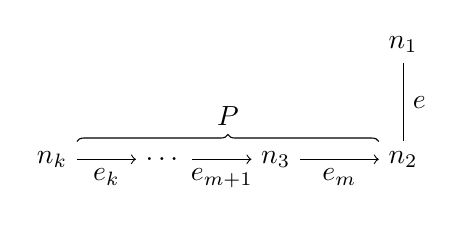
\begin{tikzpicture}
            \node (n1)                      {\(n_{1}\)};
            \node (n2) [below=1cm of n1]    {\(n_{2}\)};
            \node (n3) [left=1cm of n2]     {\(n_{3}\)};
            \node (ee) [left=0.75cm of n3]  {\ldots};
            \node (nk) [left=0.75cm of ee]  {\(n_{k}\)};
        
            \graph{
                (n1) -- [edge label={\(e\)}] (n2);
                (nk) -> [edge label={\(e_{k}\)},swap] (ee) -> [edge label={\(e_{m+1}\)},swap] (n3) -> [edge label={\(e_{m}\)},swap] (n2);
            };
            
            \node (Pleft) [above=2mm of nk.north east] {};
            \node (Pright) [above=2mm of n2.north west] {};
            \node (P) at ($(Pleft)!0.5!(Pright)$) {\(P\)};
            \draw[decorate,decoration=brace] (nk.north east) -- (n2.north west);
        \end{tikzpicture}
    }
    
    \subfloat[Copy edge \(e\) to \(e'\) across path \(P\)\label{fig-sig-composition-copy}]{
        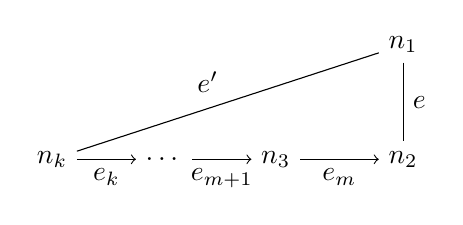
\begin{tikzpicture}
            \node (n1)                      {\(n_{1}\)};
            \node (n2) [below=1cm of n1]    {\(n_{2}\)};
            \node (n3) [left=1cm of n2]     {\(n_{3}\)};
            \node (ee) [left=0.75cm of n3]  {\ldots};
            \node (nk) [left=0.75cm of ee]  {\(n_{k}\)};
        
            \graph{
                (n1) -- [edge label={\(e\)}]        (n2);
                (n1) -- [edge label={\(e'\)},swap]  (nk);
                (nk) -> [edge label={\(e_{k}\)},swap] (ee) -> [edge label={\(e_{m+1}\)},swap] (n3) -> [edge label={\(e_{m}\)},swap] (n2);
            };
        \end{tikzpicture}
    }
    
    \subfloat[Move edge \(e\) to \(e'\) across path \(P\)\label{fig-sig-composition-move}]{
        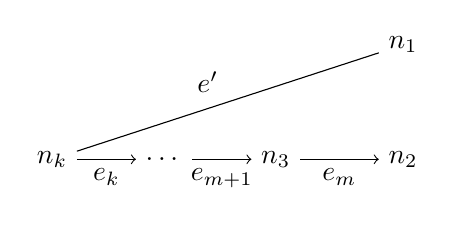
\begin{tikzpicture}
            \node (n1)                      {\(n_{1}\)};
            \node (n2) [below=1cm of n1]    {\(n_{2}\)};
            \node (n3) [left=1cm of n2]     {\(n_{3}\)};
            \node (ee) [left=0.75cm of n3]  {\ldots};
            \node (nk) [left=0.75cm of ee]  {\(n_{k}\)};
        
            \graph{
                (n1) -- [edge label={\(e'\)},swap]  (nk);
                (nk) -> [edge label={\(e_{k}\)},swap] (ee) -> [edge label={\(e_{m+1}\)},swap] (n3) -> [edge label={\(e_{m}\)},swap] (n2);
            };
        \end{tikzpicture}
    }
    \caption{Composition transformations.}
    \label{fig-sig-composition}
\end{figure}

%%%%%%%%%%%%%%%%%%%%

    \item[Selection transformations] allow the creation and deletion of new nodes and edges as follows:
    \begin{enumerate}
        
        \item An existing node \(n\) may be duplicated to create a new node \(n'\!\). A trivial selection edge \(e:n \TrivialSelection n'\) is added to enforce the constraint that \(n'\) is a duplicate of \(n\).
        
        \item A node \(n_{1}\) may be deleted if it is associated with exactly one other node \(n_{2}\) by a single trivial selection edge \(e:n_{1} \TrivialSelection n_{2}\) (implying \(n_{1}\) is a duplicate of \(n_{2}\)). This also deletes the trivial selection edge.
        
        \item A trivial selection edge \(e:n \TrivialSelection n\) may be created that connects a node \(n\) to itself.
        
        \item A trivial selection edge \(e:n_{1} \TrivialSelection n_{2}\) may be deleted, removing the association between \(n_{1}\) and \(n_{2}\).
        
    \end{enumerate}
    
    If we can make \(G_{\SC{1}}\) isomorphic to \(G_{\SC{2}}\) using any of the first three selection transformations, then \Equivalent{\SC{1}}{\SC{2}}. If we can make \(G_{\SC{1}}\) isomorphic to \(G_{\SC{2}}\) using the fourth selection transformation, then \Dominates{\SC{2}}{\SC{1}}. The latter may seem somewhat counter-intuitive \cite{Qian.X-1995a-Correct}, but is nonetheless correct \cite{Miller.R-1994a-Schema}. A trivial selection edge \(e:n_{1} \TrivialSelection n_{2}\) denotes that \(n_{1}\) and \(n_{2}\) correspond to the same domain, so removing the edge also removes this constraint. The information capacity of \(\SC{2}\) must therefore be greater than \(\SC{1}\).
    
\end{description}

These SIG transformations and their effects are summarised in Table~\ref{Tab.SIG.Transformations}.

%%%%%%%%%%%%%%%%%%%%

\begin{table}[htb]
    \centering
    \small
    \begin{tabular}{lcc}
        \toprule
                                                        &                   &   \textbf{Effect on infor-}   \\
        \textbf{Transformation}                         &   \textbf{Type}   &   \textbf{mation capacity}    \\
        \midrule
        Delete annotation or \(\RelProject\)/\(\RelRestrict\) constraint    &   annotation      &   augmented   \\
        Move or copy edge                               &   composition     &   augmented   \\
        Create or delete duplicate node                 &   selection       &   no change   \\
        Create trivial selection edge                   &   selection       &   no change   \\
        Delete trivial selection edge                   &   selection       &   augmented   \\
        \bottomrule
    \end{tabular}
    \caption{Summary of SIG transformations.}
    \label{Tab.SIG.Transformations}
\end{table}

%%%%%%%%%%%%%%%%%%%%

%%%%%%%%%%%%%%%%%%%%%%%%%%%%%%%%%%%%%%%%%%%%%%%%%%%%%%%%%%%%%%%%%%%%%%%%%%%%%%%%%


\section{Extending SIGs to model relational concepts}
\label{sec-relational-sigs}

\noindent The direct correspondence between relational types and SIG domains noted in Section~\ref{sec-relations-types} enables us to use SIGs to represent the structure and constraints of relational schemas. Equating tuple types to the Cartesian product of their attributes (equation \ref{eqn-tuple-type}) means that these can also be mapped directly to a constructed SIG node.

Let us again consider the relvar \(S\{\Sno, \Sname, \Status, \City\}\) from Date's suppliers-and-parts schema \cite{Date.C-2013a-View}. In addition to type constraints on the attributes, tuples, and the relvar as a whole, \(S\) is subject to a (primary) key constraint on \Sno. Taken together with the collection of types \(\Type{\Sno}\), \(\Type{\Sname}\), \(\Type{\Status}\), \(\Type{\City}\), \(\TT{S}\), and \(\Type{S}\), and assuming that \(S\) is the only relvar in the schema, we can construct the SIG shown in Figure~\ref{fig-sig-s-alone} as explained below.

%%%%%%%%%%%%%%%%%%%%

\begin{figure}[htb]
    \centering
    \begin{tikzpicture}[level distance=12mm]
        \node (TS) {\(\Type{S}\)};
        \node (TTS) [right=1cm of TS] {\(\TT{S}\)}
            [sibling distance=3cm]
            child[arrows={<{crossbar}-{crossbar}>}] {node (TSno) {\(\Type{\Sno}\)}}
            child[arrows={:{crossbar}-{crossbar}>}] {node (TSSC) {\(\TSSC\)}
                [sibling distance=15mm]
                child[arrows={:{crossbar}-{crossbar}>}] {node (TSname) {\(\Type{\Sname}\)}}
                child[arrows={:{crossbar}-{crossbar}>}] {node (TStatus) {\(\Type{\Status}\)}}
                child[arrows={:{crossbar}-{crossbar}>}] {node (TCity) {\(\Type{\City}\)}}};
        
        % TS to T{S}
        \draw[arrows={:{crossbar}-{crossbar}:}] (TS) to (TTS);
        
        % FD
        \draw[arrows={:{crossbar}-{crossbar}>}] (TSno) to node[below=-2pt] {\scriptsize\emph{key}} (TSSC);
        
        % projection edges
        \ProjectionAnnotation[above left=-2pt and -4pt]{TTS}{TSno}
        \ProjectionAnnotation[above right=-2pt and -4pt]{TTS}{TSSC}

        \ProjectionAnnotation[above left=-2pt and -4pt]{TSSC}{TSname}
        \ProjectionAnnotation[right=-2pt]{TSSC}{TStatus}
        \ProjectionAnnotation[above right=-2pt and -4pt]{TSSC}{TCity}
    \end{tikzpicture}
    \caption{SIG for relvar \(S\{\Sno, \Sname, \Status, \City\}\).}
    \label{fig-sig-s-alone}
\end{figure}

%%%%%%%%%%%%%%%%%%%%

As discussed in Section~\ref{sec-relations-types}, any given value of \(S\) must comprise a subset of \(\TT{S}\), so the association between \(\Type{S}\) and \(\TT{S}\) is total. Similarly, every tuple in \(\TT{S}\) must appear in at least one value of \(S\), so the association is also surjective. The association is neither functional nor injective, however, as a value of \(S\) in general may contain multiple tuples, and each tuple in \(\TT{S}\) can appear in multiple values of \(S\). This gives us \(\Type{S}\SurTotal\TT{S}\).
    
The key constraint on \Sno\ implies that the functional dependency \(\{\Sno\} \rightarrow \{\Sname, \Status, \City\}\) holds in \(S\). From equation \ref{eqn-tuple-type}, we can infer the type of \(\{\Sname, \Status, \City\}\) as \(\TSSC\). The association is functional and not injective by definition. Every supplier number (when used in a value of \(S\)) must be associated with an element of \(\TSSC\), and vice versa. This implies that the association is both total and surjective. Indeed, this holds for every edge that represents a key constraint \cite{Miller.R-1994a-SIG}. We introduce the edge label \(\mathit{key}\) to denote an edge representing a key constraint, which gives us \(\Type{\Sno} \KeyEdge \TSSC\) in Figure~\ref{fig-sig-s-alone}. 
    
Both \(\Type{\Sno}\) and \(\TSSC\) are projections of \(\TT{S}\), so we can add a non-unique projection edge \(\TT{S} \ProjectionEdge \Type{\Sname} \times \Type{\Status} \times T_{\City}\) and a unique projection edge \(\TT{S} \TrivialProjection \Type{\Sno}\). Similarly, \(\Type{\Sname}\), \(\Type{\Status}\), and \(\Type{\City}\) are all projections of \(\TSSC\), so we can add further non-unique projection edges to these nodes, as shown in Figure~\ref{fig-sig-s-alone}.

Looking at Figure~\ref{fig-sig-s-alone}, it could be argued that the \(T_{\dots}\) type notation is redundant and unnecessarily complicates the diagram. Why not just use, e.g., \(S\) instead of \(\Type{S}\), \(\Sno\) instead of \(\Type{\Sno}\), and \(\Sno \times \Sname \times \Status \times \City\) instead of \(\TT{S}\)? It is important to remember, however, that SIGs like that shown in Figure~\ref{fig-sig-s-alone} refer to multiple elements of quite different kinds, including relations, tuples, and various combinations of attributes. Discarding the type notation might be reasonable in informal situations, but could lead to confusion between the different kinds of elements represented. The explicit type notation protects the semantics of the various elements of the schema and makes it clear what is being represented.


%%%%%%%%%%%%%%%%%%%%%%%%%%%%%%%%%%%%%%%%%%%%%%%%%%%%%%%%%%%%%%%%%%%%%%%%%%%%%%%%%


\section{Characterising view updates}
\label{sec-characterising}

\noindent In this section we show how the extended SIG formalism can be used to model the information equivalence of relational view updates, using Date's restriction view example as a proof of concept \cite{Date.C-2013a-View}.

Views and the base relvars they are derived from normally exist within the same ``base'' database schema (although this is not strictly required), which we shall refer to as \(\SC{0}\). However, an end user may be granted access only to the views, and thus not be aware of the existence of the base relvar(s), or vice versa. This effectively partitions the schema into logical sub-schemas \(\SC{1}, \SC{2}, \dotsc, \SC{n}\).

There are explicit and implicit constraints in \(\SC{0}\) that should also apply to the sub-schemas \cite{Date.C-2013a-View}. Ignoring these constraints in a sub-schema \(\SC{k}\) will affect its information capacity, and could negatively impact the information equivalence of view updates involving \(\SC{k}\). In the next section we will show how such constraints can be propagated into sub-schemas by rewriting them in terms of the sub-schema alone, which enables us to explicitly incorporate into the sub-schema semantic information implicit in \(\SC{0}\) that would otherwise be lost. We will then discuss the construction of SIGs for Date's restriction view example (Section~\ref{sec-date-sigs}), and show how to transform and compare these (Section~\ref{sec-transforming}).


%%%%%%%%%%%%%%%%%%%%%%%%%%%%%%%%%%%%%%%%%%%%%%%%%%%%%%%%%%%%%%%%%%%%%%%%%%%%%%%%%


\subsection{Constraint derivation and propagation}
\label{sec-constraints}

\noindent Date's motivating example in Chapter 4 of \cite{Date.C-2013a-View} explores what is arguably the simplest case of view updating: disjoint restriction views. The example includes a base relvar \(S\) and two views \(\LS\) and \(\NLS\) derived\footnote{Although as Date notes \cite{Date.C-2013a-View}, we could just as easily define \(\LS\) and \(\NLS\) as base relvars and then derive \(S = \LS \RelUnion \NLS\), or even define all three as base relvars. The constraints remain the same regardless.} from \(S\):
\begin{align}
    \LS  &= \RelRestrict_{\City = \mathit{'London'}}S \label{eqn-ls}   \\
    \NLS &= \RelRestrict_{\City \ne \mathit{'London'}}S \label{eqn-nls}
\end{align}

Informally, \(\LS\) and \(\NLS\) contain details of London and non-London suppliers, respectively. They represent disjoint restrictions of \(S\) with the same heading, and have the following tuple types:
\begin{align}
    \TT{\LS}  &= \Type{\Sno} \times \Type{\Sname} \times \Type{\Status} \times \CityLondon \nonumber    \\
    \TT{\NLS} &= \Type{\Sno} \times \Type{\Sname} \times \Type{\Status} \times (\TCityMinusLondon) \nonumber
\end{align}

The base schema for this example is \(\SC{0} = \{S, \LS, \NLS\}\). This is subject to type constraints as specified by the various types noted previously, and the following additional constraints:
\begin{ConstraintList}

    \item\label{constraint-key} \Sno\ is a key for each of \(S\), \(\LS\), and \(\NLS\), therefore the functional dependency \(\{\Sno\} \rightarrow \{\Sname, \Status, \City\}\) also holds in each of (a) \(S\); (b) \(\LS\); and (c) \(\NLS\).
    
    % not sure how relevant the FK constraints are?
    % how to represent? FK is a subset of the original key, so selection edge between S.Sno and each of LS.Sno and NLS.Sno
    % or perhaps a selection edge from Sno to itself? (labelled FK)
    % Notation: \Type{\Sno}, \Type{\LS.\Sno}, \Type{\NLS.\Sno}?
    \item\label{constraint-lsfk} \(\RelProject_{\{\Sno\}}\LS \subseteq \RelProject_{\{\Sno\}}S\) [foreign key from \(\LS\) to \(S\)]
    
    \item\label{constraint-nlsfk} \(\RelProject_{\{\Sno\}}\NLS \subseteq \RelProject_{\{\Sno\}}S\) [foreign key from \(\NLS\) to \(S\)]
    
    \item\label{constraint-union} \(S = \LS \RelUnion \NLS\) [from (\ref{eqn-ls}) and (\ref{eqn-nls}) above]
    
    \item\label{constraint-notlondon} \(\RelRestrict_{\City \ne \mathit{'London'}}\LS = \emptyset\) [from (\ref{eqn-ls}) above]
    
    \item\label{constraint-london} \(\RelRestrict_{\City = \mathit{'London'}}\NLS = \emptyset\) [from (\ref{eqn-nls}) above]
    
    \item\label{constraint-disjoint} \(\LS \RelIntersect \NLS = \emptyset\) [from \Constraint{\ref{constraint-notlondon}} and \Constraint{\ref{constraint-london}}]
    
    \item\label{constraint-relation-type-union} (a) \(\Type{S} = \Type{\LS} \RelUnion \Type{\NLS}\); (b) \(\TT{S} = \TT{\LS} \RelUnion \TT{\NLS}\) [from \Constraint{\ref{constraint-union}}]
    
    \item\label{constraint-relation-types} (a) \(\Type{\LS} \subset \Type{S}\); (b) \(\TT{\LS} \subset \TT{S}\) [from (\ref{eqn-ls}) above]
    
    \item\label{constraint-tuple-types} (a) \(\Type{\NLS} \subset \Type{S}\); (b) \(\TT{\NLS} \subset \TT{S}\) [from (\ref{eqn-nls}) above]
    
    \item\label{constraint-implied-types-london} \(\CityLondon \subset \Type{\City}\)
    
    \item\label{constraint-implied-types-nonlondon} \((\TCityMinusLondon) \subset \Type{\City}\)
    
    \item\label{constraint-implied-types-TSSL} \(\TSSL \subset \TSSC\)
    
    \item\label{constraint-implied-types-TSSNL} \(\TSSNL \subset \TSSC\)
    
\end{ConstraintList}

Constraints \Constraint{\ref{constraint-union}}--\Constraint{\ref{constraint-disjoint}} enforce that \(\LS\) and \(\NLS\) are disjoint restrictions of \(S\), while \Constraint{\ref{constraint-relation-type-union}}--\Constraint{\ref{constraint-implied-types-TSSNL}} are additional type constraints that enforce specialisation associations implied by the subtypes and supertypes occurring in \(\SC{0}\).

In most typical database schemas, only constraints \Constraint{\ref{constraint-key}}, \Constraint{\ref{constraint-lsfk}}, and \Constraint{\ref{constraint-nlsfk}} will be explicitly declared. Some database schemas may also explicitly declare constraints \Constraint{\ref{constraint-union}} and \Constraint{\ref{constraint-disjoint}}, but it is more likely that these and all the remaining constraints will be implicit in the definition of \(\SC{0}\). It is important for the purposes of this analysis to clearly identify all such implicit constraints, so that nothing is missed when constructing corresponding SIGs.

Let us partition \(\SC{0}\) into three sub-schemas: \(\SC{1} = \{S\}\), \(\SC{2} = \{\LS, \NLS\}\), and \(\SC{3} = \{LS\}\). We wish to compare the relative information capacities of \((\SC{1}, \SC{2})\) and \((\SC{1}, \SC{3})\), in order to characterise the view update compatibility of the schemas in each pair.

Note that in the following analysis, we omit the foreign key constraints \Constraint{\ref{constraint-lsfk}} and \Constraint{\ref{constraint-nlsfk}}, as we have yet to determine the best way to represent inclusion dependencies of this nature in a SIG\footnote{Miller et al.\ \cite{Miller.R-1994a-SIG} briefly mention inclusion dependencies, but do not discuss how to represent them in a SIG.}, or indeed whether such dependencies are significant.

%%%%%%%%%%%%%%%%%%%%

\begin{table*}
    \centering
    \begin{tabular}{cl}
        \toprule
        \textbf{Constraint}                                     &   \textbf{Implied edge(s)}    \\
        \midrule
        {\Constraint[\SC{1}]{\ref{constraint-key}}}(b)          &   \(\Type{\Sno} \KeyEdge \TSSL\)   \\
        \phantom{\Constraint[\SC{1}]{\ref{constraint-key}}}(c)  &   \(\Type{\Sno} \KeyEdge \TSSNL\)   \\
        \midrule
        {\Constraint[\SC{1}]{\ref{constraint-relation-types}}}  &   \(\Type{\LSsub} \SurTotal \TT{\LSsub}\) \quad\quad \(\Type{S} \SelectionEdge \Type{\LSsub}\) \quad\quad \(\TT{S} \SelectionEdge \TT{\LSsub}\)   \\
        \midrule
        {\Constraint[\SC{1}]{\ref{constraint-tuple-types}}}     &   \(\Type{\NLSsub} \SurTotal \TT{\NLSsub}\) \quad\quad \(\Type{S} \SelectionEdge \Type{\NLSsub}\) \quad\quad \(\TT{S} \SelectionEdge \TT{\NLSsub}\)   \\
        \midrule
        {\Constraint{\ref{constraint-implied-types-london}}}    &   \(\Type{\City} \SelectionEdge \CityLondon\)   \\
        \midrule
        {\Constraint{\ref{constraint-implied-types-nonlondon}}} &   \(\Type{\City} \SelectionEdge (\TCityMinusLondon)\)   \\
        \midrule
        {\Constraint{\ref{constraint-implied-types-TSSL}}}      &   \(\TSSC \SelectionEdge \TSSL\)    \\
            &   \(\TT{\LSsub} \ProjectionEdge \TSSL\)   \\
            &   \(\TSSL \ProjectionEdge \Type{\Sname}\)   \\
            &   \(\TSSL \ProjectionEdge \Type{\Status}\)   \\
            &   \(\TSSL \ProjectionEdge\,\CityLondon\)  \\
        \midrule
        {\Constraint{\ref{constraint-implied-types-TSSNL}}}     &   \(\TSSC \SelectionEdge \TSSNL\) \\
            &   \(\TT{\NLSsub} \ProjectionEdge \TSSNL\)  \\
            &   \(\TSSNL \ProjectionEdge \Type{\Sname}\)  \\
            &   \(\TSSNL \ProjectionEdge \Type{\Status}\)  \\
            &   \(\TSSNL \ProjectionEdge \TCityMinusLondon\)  \\
        \bottomrule
    \end{tabular}
    \caption{Constraints and the SIG edges they imply for schema \(\SC{1}\).}
    \label{Tab.SIG.Implied.Edges}
\end{table*}

%%%%%%%%%%%%%%%%%%%%


%%%%%%%%%%%%%%%%%%%%%%%%%%%%%%%%%%%%%%%%%%%%%%%%%%%%%%%%%%%%%%%%%%%%%%%%%%%%%%%%%


\subsubsection{Schema \(\SC{1}\)}
\label{sec-constraints-s-i}

\noindent A user granted access only to \(\SC{1}\) can see only relvar \(S\). Constraint \Constraint{\ref{constraint-key}}(a) can be propagated directly from \(\SC{0}\) into \(\SC{1}\) as it is already expressed in terms of \(S\) only. Constraints \Constraint{\ref{constraint-implied-types-london}}--\Constraint{\ref{constraint-implied-types-TSSNL}} do not include any named relvars in \(\SC{0}\), and thus can also be propagated directly from \(\SC{0}\) into \(\SC{1}\). Constraints \Constraint{\ref{constraint-key}}(b), \Constraint{\ref{constraint-key}}(c), and \Constraint{\ref{constraint-union}}--\Constraint{\ref{constraint-tuple-types}} cannot be propagated directly from \(\SC{0}\) into \(\SC{1}\), but can all be rewritten in terms of \(S\) only, by substituting the definitions of \(\LS\) (equation~\ref{eqn-ls}) and \(\NLS\) (equation~\ref{eqn-nls}). To simplify expressions in the following discussion, we shall use \(\LSsub\) to denote \(\RelRestrict_{\City = \mathit{'London'}}S\) (\ref{eqn-ls}) and \(\NLSsub\) to denote \(\RelRestrict_{\City \ne \mathit{'London'}}S\) (\ref{eqn-nls}). (This also clearly distinguishes the substitutions from the \(\LS\) and \(\NLS\) relvars in \(\SC{0}\), \(\SC{2}\), and \(\SC{3}\).) A constraint that has been rewritten so that it can be propagated from \(\SC{0}\) into \(\SC{1}\) is denoted by, e.g., \Constraint[\SC{1}]{\ref{constraint-union}}. Consequently we can derive the following set of rewritten constraints for \(\SC{1}\):
\begin{ConstraintList}[\SC{1}]
    
    \item \Sno\ is a key for each of \(\LSsub\) and \(\NLSsub\), therefore the functional dependency \(\{\Sno\} \rightarrow \{\Sname, \Status, \City\}\) also holds in each of (b) \(\LSsub\); and (c) \(\NLSsub\). [The fact that we are dealing with two disjoint subsets of \(\City\) does not change this.]
    
    \setcounter{constraint}{3}
    \item \(S = \LSsub \RelUnion \NLSsub\) [or even just \(S = S\)]
    
    \item \(\RelRestrict_{\City \ne \mathit{'London'}}\LSsub = \emptyset\)
    
    \item \(\RelRestrict_{\City = \mathit{'London'}}\NLSsub = \emptyset\)
    
    \item \(\LSsub \RelIntersect \NLSsub = \emptyset\)

    \item (a) \(\Type{S} = \Type{\LSsub} \RelUnion \Type{\NLSsub}\); (b) \(\TT{S} = \TT{\LSsub} \RelUnion \TT{\NLSsub}\) \newline
    {[or even just \(\Type{S} = \Type{S}\) and \(\TT{S} = \TT{S}\)]}
    
    \item (a) \(\Type{\LSsub} \subset \Type{S}\); (b) \(\TT{\LSsub} \subset \TT{S}\) [from (\ref{eqn-ls}) above]
    
    \item (a) \(\Type{\NLSsub} \subset \Type{S}\); (b) \(\TT{\NLSsub} \subset \TT{S}\) [from (\ref{eqn-nls}) above]
    
\end{ConstraintList}


%%%%%%%%%%%%%%%%%%%%%%%%%%%%%%%%%%%%%%%%%%%%%%%%%%%%%%%%%%%%%%%%%%%%%%%%%%%%%%%%%


\subsubsection{Schema \(\SC{2}\)}
\label{sec-constraints-s-ii}

\noindent A user granted access only to \(\SC{2}\) can see only relvars \(\LS\) and \(\NLS\). Constraints \Constraint{\ref{constraint-key}}(b),  \Constraint{\ref{constraint-key}}(c), and \Constraint{\ref{constraint-notlondon}}--\Constraint{\ref{constraint-disjoint}} can be propagated directly from \(\SC{0}\) into \(\SC{2}\) as they are defined only in terms of \(\LS\) and \(\NLS\). \Constraint{\ref{constraint-implied-types-london}}--\Constraint{\ref{constraint-implied-types-TSSNL}} can be propagated directly into \(\SC{2}\) as they are not expressed in terms of any named relvars in \(\SC{0}\). \Constraint{\ref{constraint-key}}(a), \Constraint{\ref{constraint-union}}, \Constraint{\ref{constraint-relation-type-union}}, \Constraint{\ref{constraint-relation-types}}, and \Constraint{\ref{constraint-tuple-types}} can be rewritten in terms of \(\LS\) and \(\NLS\) only, giving us:
\begin{ConstraintList}[\SC{2}]

    \item \Sno\ is a key for \(\LS \RelUnion \NLS\), therefore the functional dependency \(\{\Sno\} \rightarrow \{\Sname, \Status, \City\}\) also holds in (a) \(\LS \RelUnion \NLS\).
    
    \setcounter{constraint}{3}
    \item \(\LS \RelUnion \NLS = \LS \RelUnion \NLS\)
    
    \setcounter{constraint}{7}
    \item (a) \(\Type{\LS} \RelUnion \Type{\NLS} = \Type{\LS} \RelUnion \Type{\NLS}\); \newline
          (b) \(\TT{\LS} \RelUnion \TT{\NLS} = \TT{\LS} \RelUnion \TT{\NLS}\)
    
    \item (a) \(\Type{\LS} \subset \Type{\LS} \RelUnion \Type{\NLS}\); (b) \(\TT{\LS} \subset \TT{\LS} \RelUnion \TT{\NLS}\)
    
    \item (a) \(\Type{\NLS} \subset \Type{\LS} \RelUnion \Type{\NLS}\); (b) \(\TT{\NLS} \subset \TT{\LS} \RelUnion \TT{\NLS}\)
    
\end{ConstraintList}


%%%%%%%%%%%%%%%%%%%%%%%%%%%%%%%%%%%%%%%%%%%%%%%%%%%%%%%%%%%%%%%%%%%%%%%%%%%%%%%%%


\subsubsection{Schema \(\SC{3}\)}
\label{sec-constraints-s-iii}

\noindent A user granted access only to \(\SC{3}\) can see only relvar \(\LS\). Constraints \Constraint{\ref{constraint-key}}(b) and \Constraint{\ref{constraint-notlondon}} can be propagated directly into \(\SC{3}\), as they are defined in terms of \(\LS\) only. \Constraint{\ref{constraint-implied-types-london}}--\Constraint{\ref{constraint-implied-types-TSSNL}} can also be propagated directly into \(\SC{3}\) as previously discussed. The remaining constraints cannot be rewritten in terms of \(\LS\) only, and so cannot be propagated into \(\SC{3}\). As we were able to propagate all constraints into \(\SC{1}\), this indicates a qualitative difference between \(\SC{1}\) and \(\SC{3}\). It therefore seems likely that the relative information capacities of \(\SC{1}\) and \(\SC{3}\) will also differ.

%%%%%%%%%%%%%%%%%%%%%%%%%%%%%%%%%%%%%%%%%%%%%%%%%%%%%%%%%%%%%%%%%%%%%%%%%%%%%%%%%


\subsection{Constructing the SIGs}
\label{sec-date-sigs}


%%%%%%%%%%%%%%%%%%%%%%%%%%%%%%%%%%%%%%%%%%%%%%%%%%%%%%%%%%%%%%%%%%%%%%%%%%%%%%%%%


\subsubsection{Schema \(\SC{1}\)}
\label{sec-sigs-s-i}

\noindent The SIG for \(\SC{1}\) will not just be that for relvar \(S\) as shown in Figure~\ref{fig-sig-s-alone}, as that schema did not incorporate all the constraints implicit in \(\SC{0}\). The process for constructing the SIG will be similar to that for the earlier example, however. The constraints appearing in \(\SC{1}\) are \Constraint{\ref{constraint-key}}(a), \Constraint[\SC{1}]{\ref{constraint-key}}(b), \Constraint[\SC{1}]{\ref{constraint-key}}(c), \Constraint[\SC{1}]{\ref{constraint-union}}--\Constraint[\SC{1}]{\ref{constraint-tuple-types}}, and \Constraint{\ref{constraint-implied-types-london}}--\Constraint{\ref{constraint-implied-types-TSSNL}}.

The SIG will include all of the edges that appear in Figure~\ref{fig-sig-s-alone}. The constraints within the schema also imply the existence of several subtype nodes (e.g., the two subtypes of \(\Type{City}\) implied by \Constraint{\ref{constraint-implied-types-london}} and \Constraint{\ref{constraint-implied-types-nonlondon}}), along with corresponding selection and projection edges, which are listed in Table~\ref{Tab.SIG.Implied.Edges} above. \Constraint[\SC{1}]{\ref{constraint-union}}, \Constraint[\SC{1}]{\ref{constraint-relation-type-union}}(a), and \Constraint[\SC{1}]{\ref{constraint-relation-type-union}}(b) are effectively tautologies that add no new information, and can thus be safely ignored. The completed SIG for \(\SC{1}\) is shown in Figure~\ref{fig-sig-s}.

%%%%%%%%%%%%%%%%%%%%

\begin{figure*}
    \centering
    \begin{tikzpicture}
        \matrix[row sep=0.5cm]
        { 
            \node (TLS) {\(\Type{\LSsub}\)};   &[7mm]  \node (TTLS) {\(\TT{\LSsub}\)};     &[7mm]                              &[4mm]                                  &[-4mm] \node (TSSL) {\(\StackTSSL\)};      &                                       &   \node (LSCity) {\(\CityLondon\)};   \\
                                            &                                           &                                   &   \node (TSname) {\(\Type{\Sname}\)};    \\
            \node (TLSPlusNLS) {\(\Type{S}\)}; &       \node (TTLSPlusNLS) {\(\TT{S}\)};   &   \node (TSno) {\(\Type{\Sno}\)};    &                                       &       \node (TSSC) {\(\StackTSSC\)};      &                                       &   \node (TCity) {\(\Type{City}\)};   \\
                                            &                                           &                                   &                                       &                                           &   \node (TStatus) {\(\Type{\Status}\)};  \\
            \node (TNLS) {\(\Type{\NLSsub}\)}; &       \node (TTNLS) {\(\TT{\NLSsub}\)};   &                                   &                                       &       \node (TSSNL) {\(\StackTSSNL\)};    &                                       &   \node (NLSCity) {\(\StackTCityMinusLondon\)}; \\
        };
        
        \graph{
            % relation types to tuple types
            { [edges=surtotal]
                { (TLS), (TNLS), (TLSPlusNLS) } -- { (TTLS), (TTNLS), (TTLSPlusNLS) },
            };
            
            % FDs
            (TSno) -- [funcdep left,bend left] (TSSL);
            (TSno) -- [funcdep right] (TSSNL);
            
            % projection edges
            { [edges=bijection,edge label={\scriptsize\(\RelProject\)}]
                { (TTLSPlusNLS), (TTLS) } -- (TSno)
            };
            
            { [edges=bijection,edge label'={\scriptsize\(\RelProject\)}]
                (TTNLS) -- (TSno)
            };
            
            { [edges=projection left]
                (TTLS)  -- (TSSL),
                (TSSL)  -- { (TStatus), (LSCity) },
            };
            
            { [edges=projection right]
                (TTNLS) -- (TSSNL),
                (TSSC)  -- { (TSname),  (TStatus) },
                (TSSL)  -- (TSname),
                (TSSNL) -- { (TStatus), (NLSCity), (TSname) },
            };
            
            % selection edges
            { [edges=selection left]
                { (TLSPlusNLS), (TTLSPlusNLS) } -- { (TLS), (TTLS) },
                (TSSC)  -- { (TSSL), (TSSNL) },
                (TCity) -- (NLSCity),
            };
            { [edges=selection right]
                { (TLSPlusNLS), (TTLSPlusNLS) } -- { (TNLS), (TTNLS) },
                (TCity) -- (LSCity),
            };
            
            % insert "gaps" into crossed edges
            { [edges={white,line width=1.5mm}]
                (TSno) -- (TSSC),
                (TSSC) -- (TCity),
                (TTLSPlusNLS) -- [bend right] (TSSC),
            };
            (TSno) -- [funcdep right] (TSSC);
            (TSSC) -- [projection left] (TCity);
            (TTLSPlusNLS) -- [projection right,bend right] (TSSC),
        };
    \end{tikzpicture}
    \caption{SIG for schema \(\SC{1} = \{S\}\).}
    \label{fig-sig-s}
\end{figure*}

%%%%%%%%%%%%%%%%%%%%

%%%%%%%%%%%%%%%%%%%%

\begin{figure*}
    \centering
    \begin{tikzpicture}
        \matrix[row sep=0.5cm]
        { 
            \node (TLS) {\(\Type{\LS}\)};                  &[7mm]  \node (TTLS) {\(\TT{\LS}\)};                    &[7mm]                              &[4mm]                                  &[-4mm] \node (TSSL) {\(\StackTSSL\)};      &                                       &   \node (LSCity) {\(\CityLondon\)};   \\
                                                        &                                                       &                                   &   \node (TSname) {\(\Type{\Sname}\)};    \\
            \node (TLSPlusNLS) {\(\StackTLSPlusNLS\)};  &       \node (TTLSPlusNLS) {\(\StackTTLSPlusNLS\)};    &   \node (TSno) {\(\Type{\Sno}\)};    &                                       &       \node (TSSC) {\(\StackTSSC\)};      &                                       &   \node (TCity) {\(\Type{City}\)};   \\
                                                        &                                                       &                                   &                                       &                                           &   \node (TStatus) {\(\Type{\Status}\)};  \\
            \node (TNLS) {\(\Type{\NLS}\)};                &       \node (TTNLS) {\(\TT{\NLS}\)};                  &                                   &                                       &       \node (TSSNL) {\(\StackTSSNL\)};    &                                       &   \node (NLSCity) {\(\StackTCityMinusLondon\)}; \\
        };
        
        \graph{
            % relation types to tuple types
            { [edges=surtotal]
                { (TLS), (TNLS), (TLSPlusNLS) } -- { (TTLS), (TTNLS), (TTLSPlusNLS) },
            };
            
            % FDs
            (TSno) -- [funcdep left,bend left] (TSSL);
            (TSno) -- [funcdep right] (TSSNL);
            
            % projection edges
            { [edges=bijection,edge label={\scriptsize\(\RelProject\)}]
                { (TTLSPlusNLS), (TTLS) } -- (TSno)
            };
            
            { [edges=bijection,edge label'={\scriptsize\(\RelProject\)}]
                (TTNLS) -- (TSno)
            };
            
            { [edges=projection left]
                (TTLS)  -- (TSSL),
                (TSSL)  -- { (TStatus), (LSCity) },
            };
            
            { [edges=projection right]
                (TTNLS) -- (TSSNL),
                (TSSC)  -- { (TSname),  (TStatus) },
                (TSSL)  -- (TSname),
                (TSSNL) -- { (TStatus), (NLSCity), (TSname) },
            };
            
            % selection edges
            { [edges=selection left]
                { (TLSPlusNLS), (TTLSPlusNLS) } -- { (TLS), (TTLS) },
                (TSSC)  -- { (TSSL), (TSSNL) },
                (TCity) -- (NLSCity),
            };
            { [edges=selection right]
                { (TLSPlusNLS), (TTLSPlusNLS) } -- { (TNLS), (TTNLS) },
                (TCity) -- (LSCity),
            };
            
            % insert "gaps" into crossed edges
            { [edges={white,line width=1.5mm}]
                (TSno) -- (TSSC),
                (TSSC) -- (TCity),
                (TTLSPlusNLS) -- [bend right] (TSSC),
            };
            (TSno) -- [funcdep right] (TSSC);
            (TSSC) -- [projection left] (TCity);
            (TTLSPlusNLS) -- [projection right,bend right] (TSSC),
        };
    \end{tikzpicture}
    \caption{SIG for schema \(\SC{2} = \{\LS, \NLS\}\).}
    \label{fig-sig-ls-nls}
\end{figure*}

%%%%%%%%%%%%%%%%%%%%

%%%%%%%%%%%%%%%%%%%%

\begin{figure*}
    \centering
    \begin{tikzpicture}
        \matrix[row sep=0.5cm]
        { 
            \node (TLS) {\(\Type{\LS}\)};  &[7.5mm]  \node (TTLS) {\(\TT{\LS}\)};  &[7mm]                              &[4mm]                                  &[-4mm] \node (TSSL) {\(\StackTSSL\)};      &                                       &   \node (LSCity) {\(\CityLondon\)};   \\
                                        &                                       &                                   &   \node (TSname) {\(\Type{\Sname}\)};    \\
                                        &                                       &   \node (TSno) {\(\Type{\Sno}\)};    &                                       &       \node (TSSC) {\(\StackTSSC\)};      &                                       &   \node (TCity) {\(\Type{City}\)};   \\
                                        &                                       &                                   &                                       &                                           &   \node (TStatus) {\(\Type{\Status}\)};  \\
                                        &                                       &                                   &                                       &       \node (TSSNL) {\(\StackTSSNL\)};    &                                       &   \node (NLSCity) {\(\StackTCityMinusLondon\)}; \\
        };
        
        \graph{
            % relation types to tuple types
            { [edges=surtotal]
                (TLS) -- (TTLS),
            };
            
            % projection edges
            { [edges=bijection,edge label={\scriptsize\(\RelProject\)}]
                (TTLS) -- (TSno)
            };
            
            { [edges=projection left]
                (TTLS)  -- (TSSL),
                (TSSL)  -- { (TStatus), (LSCity) },
            };
            
            { [edges=projection right]
                (TSSC)  -- { (TSname),  (TStatus) },
                (TSSL)  -- (TSname),
                (TSSNL) -- { (TStatus), (NLSCity), (TSname) },
            };
            
            % selection edges
            { [edges=selection left]
                (TSSC)  -- { (TSSL), (TSSNL) },
                (TCity) -- (NLSCity),
            };
            { [edges=selection right]
                (TCity) -- (LSCity),
            };
            
            % insert "gaps" into crossed edges
            { [edges={white,line width=1.5mm}]
                (TSno) -- (TSSC),
                (TSSC) -- (TCity),
            };
            (TSno) -- [funcdep right] (TSSC);
            (TSSC) -- [projection left] (TCity);
        };
    \end{tikzpicture}
    \caption{SIG for schema \(\SC{3} = \{\LS\}\).}
    \label{fig-sig-ls}
\end{figure*}

%%%%%%%%%%%%%%%%%%%%


%%%%%%%%%%%%%%%%%%%%%%%%%%%%%%%%%%%%%%%%%%%%%%%%%%%%%%%%%%%%%%%%%%%%%%%%%%%%%%%%%


\subsubsection{Schema \(\SC{2}\)}
\label{sec-sigs-s-ii}

\noindent The constraints appearing in \(\SC{2}\) are \Constraint[\SC{2}]{\ref{constraint-key}}(a), \Constraint{\ref{constraint-key}}(b), \Constraint{\ref{constraint-key}}(c), \Constraint[\SC{2}]{\ref{constraint-union}}, \Constraint{\ref{constraint-notlondon}}--\Constraint{\ref{constraint-disjoint}}, \Constraint[\SC{2}]{\ref{constraint-relation-type-union}}--\Constraint[\SC{2}]{\ref{constraint-tuple-types}}, and \Constraint{\ref{constraint-implied-types-london}}--\Constraint{\ref{constraint-implied-types-TSSNL}}. This is essentially the same set of constraints as \(\SC{1}\), but with different rewritings. This means that the SIG for \(\SC{2}\) can be built in the same manner as for \(\SC{1}\), with some nodes named differently. In particular, \Constraint[\SC{2}]{\ref{constraint-relation-type-union}} implies that there will be nodes \(\TLSPlusNLS\) and \(\TTLSPlusNLS\) instead of \(\Type{S}\) and \(\TT{S}\), respectively. There will also be \(\Type{\LS}\) instead of \(\Type{\LSsub}\), etc. The complete SIG for \(\SC{2}\) is shown in Figure~\ref{fig-sig-ls-nls}.


%%%%%%%%%%%%%%%%%%%%%%%%%%%%%%%%%%%%%%%%%%%%%%%%%%%%%%%%%%%%%%%%%%%%%%%%%%%%%%%%%


\subsubsection{Schema \(\SC{3}\)}
\label{sec-sigs-s-iii}

\noindent The constraints appearing in \(\SC{3}\) are \Constraint{\ref{constraint-key}}(b), \Constraint{\ref{constraint-notlondon}}, and \Constraint{\ref{constraint-implied-types-london}}--\Constraint{\ref{constraint-implied-types-TSSNL}}. The SIG will only include edges and nodes that relate either directly to \(\LS\) or are independent of any relvar, such as the subtype node \(\TSSNL\). The complete SIG for \(\SC{3}\) is shown in Figure~\ref{fig-sig-ls} on the previous page.


%%%%%%%%%%%%%%%%%%%%%%%%%%%%%%%%%%%%%%%%%%%%%%%%%%%%%%%%%%%%%%%%%%%%%%%%%%%%%%%%%


\subsection{Transforming the SIGs}
\label{sec-transforming}

\noindent Now that we have constructed SIGs for all three schemas, we can compare the relative information capacities of the schema pairs \((\SC{1}, \SC{2})\) and \((\SC{1}, \SC{3})\). We do this by attempting to transform the SIG for one of the schemas until it is isomorphic with the other.

Looking at the SIGs for \(\SC{1}\) and \(\SC{2}\), we can see almost immediately that both SIGs have the same node and edge structure; indeed the only difference is in the names of some of the nodes. However, we already know from the discussion in Sections~\ref{sec-constraints-s-i} and~\ref{sec-constraints-s-ii} that these differently named nodes are just rewritings that represent the same domains. We therefore have an immediate isomorphism between the two SIGs and can conclude that the information capacities of \(\SC{1}\) and \(\SC{2}\) are equivalent, i.e., \(\Equivalent{\SC{1}}{\SC{2}}\).

The comparison between \(\SC{1}\) and \(\SC{3}\) is more interesting. There are some shared structures, but the two SIGs are clearly different. Since the SIG transformations discussed in Section~\ref{sec-sig-compare} only ever preserve or enhance information capacity, intuitively we should attempt to transform the ``smaller'' SIG for \(\SC{3}\) into the ``larger'' SIG for \(\SC{1}\). SIG transformations can generally be carried out in two broad phases (using the \(\SC{3} \rightarrow \SC{1}\) transformation as an example):
\begin{description}

    \item[Duplicate nodes] in \(\SC{3}\) (producing \(\SC{3}'\)) that correspond to supertypes in \(\SC{1}\), in order to create nodes corresponding to the extra nodes that \(\SC{1}\) has over \(\SC{3}\). The goal is to produce a node structure similar to \(\SC{1}\). The duplicated nodes are connected to their original nodes by trivial selection edges. These transformations (if applicable) do not alter the information capacity of \(\SC{3}'\) (i.e., \(\Equivalent{\SC{3}}{\SC{3}'}\)).
    
    \item[Copy and move edges] around the SIG to produce an edge structure similar to \(\SC{1}\). The annotations of each moved or copied edge are determined by the path it is composed with, as discussed in Section~\ref{sec-sig-compare}. These transformations (if applicable) \emph{increase} the information capacity of \(\SC{3}'\) (i.e., \(\Dominates{\SC{3}'}{\SC{3}}\)).
    
\end{description}

These two phases generally occur in order, but may be interspersed throughout with the following:
\begin{description}

    \item[Delete duplicate nodes] in \(\SC{3}'\) that are no longer needed, especially those that do not exist in \(\SC{1}\). These transformations (if applicable) do not alter the information capacity of \(\SC{3}'\) (\(\equiv\)).
    
    \item[Remove totality annotations] from trivial selection edges in \(\SC{3}'\) to change them into non-trivial selection edges. This decouples duplicate nodes into subtypes and supertypes, ensuring that they represent different domains. These transformations (if applicable) \emph{increase} the information capacity of \(\SC{3}'\) (\(\preceq\)).
    
\end{description}
For example, we might duplicate some nodes, remove some totality annotations, move or copy some edges, delete some no longer needed nodes, move or copy some more edges, then remove some more totality annotations.

Applying this process to \(\SC{3}\), we first duplicate node \(\Type{\LS}\) to \(\Type{S}\) and node \(\TT{\LS}\) to \(\TT{S}\). To obtain a node structure similar to that of \(\SC{1}\), we also need to further duplicate \(\Type{S}\) to \(\Type{\NLS}\) and \(\TT{S}\) to \(\TT{\NLS}\). The result of these duplications is shown in Figure~\ref{fig-transform-all-duplicates}. The transformed SIG now has the same node structure as that for \(\SC{1}\).

%%%%%%%%%%%%%%%%%%%%

\begin{figure*}[t]
    \centering
    \begin{tikzpicture}
        \matrix[row sep=0.5cm]
        { 
            \node [input keep] (TLS) {\(\Type{\LS}\)};     &[7mm]  \node [input keep] (TTLS) {\(\TT{\LS}\)};   &[7mm]                              &[4mm]                                  &[-4mm] \node (TSSL) {\(\StackTSSL\)};      &                                       &   \node (LSCity) {\(\CityLondon\)};   \\
                                                        &                                                   &                                   &   \node (TSname) {\(\Type{\Sname}\)};    \\
            \node [output] (TLSPlusNLS) {\(\Type{S}\)};    &       \node [output] (TTLSPlusNLS) {\(\TT{S}\)};  &   \node (TSno) {\(\Type{\Sno}\)};    &                                       &       \node (TSSC) {\(\StackTSSC\)};      &                                       &   \node (TCity) {\(\Type{City}\)};   \\
                                                        &                                                   &                                   &                                       &                                           &   \node (TStatus) {\(\Type{\Status}\)};  \\
            \node [output] (TNLS) {\(\Type{\NLS}\)};       &       \node [output] (TTNLS) {\(\TT{\NLS}\)};     &                                   &                                       &       \node (TSSNL) {\(\StackTSSNL\)};    &                                       &   \node (NLSCity) {\(\StackTCityMinusLondon\)}; \\
        };
        
        \graph{
            % relation types to tuple types
            { [edges=surtotal]
                (TLS) -- (TTLS),
            };
            
            % projection edges
            { [edges=bijection,edge label={\scriptsize\(\RelProject\)}]
                (TTLS) -- (TSno)
            };
            
            { [edges=projection left]
                (TTLS)  -- (TSSL),
                (TSSL)  -- { (TStatus), (LSCity) },
            };
            
            { [edges=projection right]
                (TSSC)  -- { (TSname),  (TStatus) },
                (TSSL)  -- (TSname),
                (TSSNL) -- { (TStatus), (NLSCity), (TSname) },
            };
            
            % selection edges
            { [edges=selection left]
                (TSSC)  -- { (TSSL), (TSSNL) },
                (TCity) -- (NLSCity),
            };
            { [edges=selection right]
                (TCity) -- (LSCity),
            };
            
            { [edges={bijection,output},edge label'={\scriptsize\(\RelRestrict\)}]
                { (TLS), (TTLS) } -- { (TLSPlusNLS), (TTLSPlusNLS) },
                { (TLSPlusNLS), (TTLSPlusNLS) } -- { (TNLS), (TTNLS) },
            };
            
            % insert "gaps" into crossed edges
            { [edges={white,line width=1.5mm}]
                (TSno) -- (TSSC),
                (TSSC) -- (TCity),
            };
            (TSno) -- [funcdep right] (TSSC);
            (TSSC) -- [projection left] (TCity);
            
            % transformation indicators
            { [edges={->,gray,dashed,bend left=45}]
                (TLS) -- [edge node={node[sloped,above]{\small\emph{copy}}}] (TLSPlusNLS),
                (TLSPlusNLS) -- [edge node={node[sloped,above,rotate=180]{\small\emph{copy}}}] (TNLS)
            };
        };
    \end{tikzpicture}
    \caption{SIG for transformed schema \(\SC{3}'\) after duplicating \Type{\LS} and \TT{\LS} to produce analogues of the additional nodes in \(\SC{1}\). Inputs to the transformations are coloured \textcolor{blue}{blue}, outputs are coloured \textcolor{red}{red}. [\(\equiv\)]}
    \label{fig-transform-all-duplicates}
\end{figure*}

%%%%%%%%%%%%%%%%%%%%

The next phase is to copy and move edges. To produce the edge \(\Type{S} \SurTotal \TT{S}\), we can first \emph{copy} \(\Type{\LS} \SurTotal \TT{\LS}\) across the path \(\TT{S} \TrivialSelection \TT{\LS}\) (giving \(\Type{\LS} \SurTotal \TT{S}\)), then \emph{move} it across \(\Type{S} \TrivialSelection \Type{\LS}\). We can carry out a similar series of transformations to copy and move \(\Type{S} \SurTotal \TT{S}\) to \(\Type{\NLS} \SurTotal \TT{\NLS}\) (see Figure~\ref{fig-transform-edge-moves}).

We next copy and move the unique projection edge \(\TT{\LS} \TrivialProjection \Type{\Sno}\) to produce the edges \(\TT{S} \TrivialProjection \Type{\Sno}\) and \(\TT{\NLS} \TrivialProjection \Type{\Sno}\). Similarly, we copy and move \(\TT{\LS} \ProjectionEdge \TSSL\) to produce \(\TT{S} \LabelledEdge{\sigedge{12}}{\RelProject} \TSSC\) and \(\TT{\NLS} \LabelledEdge{\sigedge{02}}{\RelProject} \TSSNL\). Note that the first edge in the latter pair of transformations loses its totality annotation, and the second edge its surjectivity annotation, as a result of composition with the pre-existing non-bijective selection edges between the constructed tuple types running vertically down the centre of the SIG.

Finally, we carry out similar copy and move transformations to copy the key edge \(\Type{\Sno} \KeyEdge \TSSC\) to \(\Type{\Sno} \LabelledEdge{\sigedge{03}}{\mathit{key}} \TSSL\), and \(\Type{\Sno} \LabelledEdge{\sigedge{03}}{\mathit{key}} \TSSNL\). Both new edges lose their totality annotations for the same reason as the projection edges above. The final result of all these edge transformations is shown in Figure~\ref{fig-transform-edge-moves}.

%%%%%%%%%%%%%%%%%%%%

\begin{figure*}[t]
    \centering
    \begin{tikzpicture}
        \matrix[row sep=0.5cm]
        { 
            \node (TLS) {\(\Type{\LS}\)};      &[7mm]  \node (TTLS) {\(\TT{\LS}\)};        &[7mm]                              &[4mm]                                  &[-4mm] \node (TSSL) {\(\StackTSSL\)};      &                                       &   \node (LSCity) {\(\CityLondon\)};   \\
                                            &                                           &                                   &   \node (TSname) {\(\Type{\Sname}\)};    \\
            \node (TLSPlusNLS) {\(\Type{S}\)}; &       \node (TTLSPlusNLS) {\(\TT{S}\)};   &   \node (TSno) {\(\Type{\Sno}\)};    &                                       &       \node (TSSC) {\(\StackTSSC\)};      &                                       &   \node (TCity) {\(\Type{City}\)};   \\
                                            &                                           &                                   &                                       &                                           &   \node (TStatus) {\(\Type{\Status}\)};  \\
            \node (TNLS) {\(\Type{\NLS}\)};    &       \node (TTNLS) {\(\TT{\NLS}\)};      &                                   &                                       &       \node (TSSNL) {\(\StackTSSNL\)};    &                                       &   \node (NLSCity) {\(\StackTCityMinusLondon\)}; \\
        };
        
        \graph{
            % relation types to tuple types
            { [edges=surtotal]
                (TLS)        -- [input keep,edge node={node (c1a) {}}] (TTLS),
                (TLSPlusNLS) -- [output,edge node={node (c1b) {}}]     (TTLSPlusNLS),
                (TNLS)       -- [output,edge node={node (c1c) {}}]     (TTNLS),
            };
            
            % FDs
            (TSno) -- [funcdep left,arrows={-{crossbar}>},bend left,output] (TSSL);
            (TSno) -- [funcdep right,arrows={-{crossbar}>},output] (TSSNL);
            
            % projection edges
            { [edges=bijection,edge label={\scriptsize\(\RelProject\)}]
                (TTLS)        -- [input keep] (TSno),
                (TTLSPlusNLS) -- [output] (TSno),
            };
            
            { [edges=bijection,edge label'={\scriptsize\(\RelProject\)}]
                (TTNLS)       -- [output] (TSno),
            };
            
            { [edges=projection left]
                (TTLS)  -- [input keep,edge node={node (c2a) {}}] (TSSL),
                (TSSL)  -- { (TStatus), (LSCity) },
            };
            
            { [edges=projection right]
                (TSSC)   -- { (TSname),  (TStatus) },
                (TSSL)   -- (TSname),
                (TSSNL)  -- { (TStatus), (NLSCity), (TSname) },
                (TTNLS)  -- [arrows={:->},output,edge node={node (c2c) {}}] (TSSNL),
            };

            % selection edges
            { [edges=selection left]
                (TSSC)  -- { (TSSL), (TSSNL) },
                (TCity) -- (NLSCity),
            };
            { [edges=selection right]
                (TCity) -- (LSCity),
            };
            
            { [edges=bijection,edge label'={\scriptsize\(\RelRestrict\)}]
                { (TLS), (TTLS) }               -- { (TLSPlusNLS), (TTLSPlusNLS) },
                { (TLSPlusNLS), (TTLSPlusNLS) } -- { (TNLS), (TTNLS) },
            };
            
            % insert "gaps" into crossed edges
            { [edges={white,line width=1.5mm}]
                (TSno) -- (TSSC),
                (TSSC) -- (TCity),
                (TTLSPlusNLS) -- [bend right] (TSSC),
            };
            (TSno) -- [funcdep right,input keep] (TSSC);
            (TSSC) -- [projection left] (TCity);
            (TTLSPlusNLS) -- [projection right,arrows={:{crossbar}->},bend right,output,edge node={node (c2b) {}}] (TSSC),
            
            % transformation indicators
            { [edges={->,gray,dashed}]
                (c1a) -- (c1b),
                (c1a) -- [bend right=12,edge node={node[above,sloped,pos=0.175]{\small\emph{copy \& move}}}] (c1c),
                (c2a) -- [bend right=12] (c2b),
                (c2a) -- [bend right=12,edge node={node[above,sloped,pos=0.175]{\small\emph{copy \& move}}}] (c2c)
            };
        };
    \end{tikzpicture}
    \caption{SIG for transformed schema \(\SC{3}'\) after copying and moving various edges. [\(\preceq\)]}
    \label{fig-transform-edge-moves}
\end{figure*}

%%%%%%%%%%%%%%%%%%%%

If we compare Figure~\ref{fig-sig-s} with Figure~\ref{fig-transform-edge-moves}, we can see that the transformed SIG for \(\SC{3}'\) now has the same topology as the SIG for \(\SC{1}\). We still need to remove the totality annotations from the newly created trivial selection edges between the relation and tuple types on the left, but even when this is done, we do not achieve the desired isomorphism, as the edges \(\TT{S} \LabelledEdge{\sigedge{12}}{\RelProject} \TSSC\), \(\TT{\NLS} \LabelledEdge{\sigedge{02}}{\RelProject} \TSSNL\), \(\Type{\Sno} \LabelledEdge{\sigedge{03}}{\mathit{key}} \TSSL\), and \(\Type{\Sno} \LabelledEdge{\sigedge{03}}{\mathit{key}} \TSSNL\) all have different annotations from the corresponding edges in the SIG for \(\SC{1}\). This clearly shows that the information capacities of \(\SC{1}\) and \(\SC{3}\) are incomparable, and that view updates based on this pair of schemas will be problematic.

If we were to create a fourth sub-schema \(\SC{4} = \{\NLS\}\) and compare this with \(\SC{1}\), the result would be similar to that for \(\SC{3}\).


%%%%%%%%%%%%%%%%%%%%%%%%%%%%%%%%%%%%%%%%%%%%%%%%%%%%%%%%%%%%%%%%%%%%%%%%%%%%%%%%%


\section{Conclusion \& future work}
\label{sec-conclusion}

\noindent In this paper we have shown how to use the concept of relative information capacity and an extension of the schema intension graph (SIG) formalism to more formally model Date's notion of information equivalence with respect to relational view updates. Our analysis of Date's restriction view example \cite{Date.C-2013a-View} using these techniques is consistent with his findings, so the approach shows promise. The information capacities of \(\SC{1} = \{S\}\) and \(\SC{2} = \{\LS,\NLS\}\) are equivalent, so it should be possible to effectively propagate view updates between \(\SC{1}\) and \(\SC{2}\), regardless of the configuration of views and base relvars. Conversely, the information capacity of \(\SC{3} = \{\LS\}\) is not comparable with that of \(\SC{1}\), implying that there are updates that cannot be propagated between \(\SC{1}\) and \(\SC{3}\).

Our analysis reinforces the importance of explicitly identifying all constraints that can be propagated from the base schema \(\SC{0}\) to its sub-schemas. Omission of constraints could produce a different SIG structure that might lead to an erroneous conclusion about a schema's information capacity relative to another.

There are several avenues for future work. First, the proof of concept discussed in this paper only deals with disjoint restriction views, which are arguably the simplest case of view updating. Further work needs to be done to characterise other types of view configuration, such as projection views, union views, and in particular, join views. This will enable us to test and refine the application of SIGs in this context.

The discussion in this paper focused only on the relational context, but relative information capacity and the SIG formalism are data model agnostic. It would therefore be interesting to investigate the application of these techniques to view updating contexts beyond the Relational Model (e.g., deductive databases).

It is unclear at present whether the omission of inclusion dependencies such as foreign keys is significant. If they are significant, the question then is how best to represent them in the SIG formalism. Adding such constraints will clearly change the structure of a SIG, but we suspect that this will not change the relationship between the relative information capacities of different schemas.

It is interesting to note that with the equivalent schemas \(\SC{1}\) and \(\SC{2}\), we were able to propagate all of the constraints from the base schema \(\SC{0}\) (Section~\ref{sec-constraints-s-ii}), whereas with the incomparable schemas \(\SC{1}\) and \(\SC{3}\), only a subset of the constraints could be propagated (Section~\ref{sec-constraints-s-iii}). A reasonable conjecture is that the degree to which constraints can be propagated from \(\SC{0}\) to its sub-schemas could be a direct indicator of information equivalence among the sub-schemas, but this needs to be further investigated.

Finally, we have recently discovered further work that explores and expands upon the concepts of information capacity and meaning within data and database schemas (e.g., \cite{Mantri.R-2010a-Data,Wang.X-2005a-SIG,Xu.K-2009a-Defining}). Some of these ideas may be applicable to our work, and need to be investigated in more detail.


%%%%%%%%%%%%%%%%%%%%%%%%%%%%%%%%%%%%%%%%%%%%%%%%%%%%%%%%%%%%%%%%%%%%%%%%%%%%%%%%%


\balance


%%%%%%%%%%%%%%%%%%%%%%%%%%%%%%%%%%%%%%%%%%%%%%%%%%%%%%%%%%%%%%%%%%%%%%%%%%%%%%%%%


\bibliographystyle{abbrv}
\bibliography{APCCM2017_Stanger}

\end{document}
